\documentclass{exam}

\newcommand{\qm}{\underline{\hspace{0.3cm}?\hspace{0.3cm}}}
\usepackage{tikz}
\usepackage{amsmath}

\begin{document}
\begin{center}
	\fbox{\fbox{\parbox{5.5in}{\centering
				Read the questions carefully. For multiple choice circle the letter corresponding to the answer}}}
\end{center}

\vspace{0.1in}
\makebox[\textwidth]{Student name:\enspace\hrulefill}

\begin{questions}
	\question What expression is another way of showing $8 \times 8$?
	\begin{choices}
		\choice $(4 \times 4 \times 4)$
		\choice $(4+4)\times 4$
		\choice $(4 \times 2) \times 8$
		\choice $(2 \times 4) + 8$
	\end{choices}

	\question The distance between two cities is 578 miles. What is the distance rounded to the nearest hundred?
	\begin{choices}
		\choice 500
		\choice 600
		\choice 580
		\choice 570
	\end{choices}

	\question What number makes the equation true $4 = \qm \div 6$ ?
	\begin{choices}
		\choice 2
		\choice 24
		\choice 12
		\choice 77
	\end{choices}

	\question There are 4 friends who each brought 3 toys to a play date Which expression can be used to find the total number of toys that were brought to the play date?
	\begin{choices}
	\choice $3 \times 4$
	\choice $3 + 4$
	\choice $4 \times 4$ 
	\choice $3 \times 3$
	\end{choices}

	\question  A rectangle can be covered completely by 10 square pieces of paper without gaps or overlaps. If each piece of paper has the side length of 2 feet, what is the total area of the rectangle?
	\begin{choices}
		\choice 40 square feet
		\choice 10 feet
		\choice 10 square feet 
		\choice 20 square feet
	\end{choices}

	\question Daniel and Jeff both run the same race.  Daniel finished 5 minutes earlier than Jeff. If Jeff finished at 3:03pm, what time did Daniel finish the race?
	\begin{choices}
		\choice 3:08 pm
		\choice 3:00 pm
		\choice 2:59 pm
		\choice 2:58 pm
	\end{choices}

	\question  The distance between Anna's home and her school is exactly 1 mile as shown on the number line below
	
	\vspace{0.1in}
	\begin{center}
	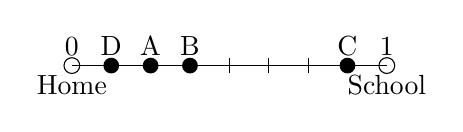
\begin{tikzpicture}
	\draw (0,0) -- (4,0);
	\draw (0,0) circle(0.1cm) node [align=center, below]{Home} node[align=center, above]{0};
%%\draw (0, -0.1) -- (0, 0.1) node[align=center, above]{0};
	\draw (0.5, -0.1) -- (0.5, 0.1);
	\draw (1, -0.1) -- (1, 0.1);
	\draw (1.5, -0.1) -- (1.5, 0.1);
	\draw (2, -0.1) -- (2, 0.1);
	\draw (2.5, -0.1) -- (2.5, 0.1);
	\draw (3, -0.1) -- (3, 0.1);
	\draw (3.5, -0.1) -- (3.5, 0.1);
	\draw (4,0) circle(0.1cm) node [align=center, below]{School} node[align=center, above]{1};
	\fill[black] (1,0) circle(0.1cm) node [align=center, above]{A};
	\fill[black] (1.5,0) circle(0.1cm) node [align=center, above]{B};
	\fill[black] (3.5,0) circle(0.1cm) node [align=center, above]{C};
	\fill[black] (0.5,0) circle(0.1cm) node [align=center, above]{D};
	\end{tikzpicture}	
    \end{center}
	Anna buys an ice cream at a store which is $\frac{1}{8}$ miles from home. What point on the number line shows the location of the store?
	\begin{choices}
		\choice Point A
		\choice Point B
		\choice Point C
		\choice Point D
	\end{choices}
	
	
	\question What number line shows the fraction $\frac{3}{4}$ correctly?
	\begin{choices}
	\choice 
	\begin{tikzpicture}
	\draw (0,0) -- (4,0);
	%%\draw (0, -0.1) -- (0, 0.1) node[align=center, above]{0};
	\draw (0, -0.1) -- (0, 0.1) node[align=center, below, yshift=-0.2cm]{0};
	\draw (0.5, -0.1) -- (0.5, 0.1);
	\draw (1, -0.1) -- (1, 0.1);
	\draw (1.5, -0.1) -- (1.5, 0.1);
	\draw (2, -0.1) -- (2, 0.1) node[align=center, below, yshift=-0.2cm]{$\frac{3}{4}$};
	\draw (2.5, -0.1) -- (2.5, 0.1);
	\draw (3, -0.1) -- (3, 0.1);
	\draw (3.5, -0.1) -- (3.5, 0.1);
	\draw (3.5, -0.1) -- (3.5, 0.1) ;
	\draw (4, -0.1) -- (4, 0.1) node[align=center, below, yshift=-0.2cm]{1};
	\end{tikzpicture}	
	\choice
	\begin{tikzpicture}
	\draw (0,0) -- (4,0);
	%%\draw (0, -0.1) -- (0, 0.1) node[align=center, above]{0};
	\draw (0, -0.1) -- (0, 0.1) node[align=center, below, yshift=-0.2cm]{0};
	\draw (0.5, -0.1) -- (0.5, 0.1)  node[align=center, below, yshift=-0.2cm]{$\frac{3}{4}$};
	\draw (1, -0.1) -- (1, 0.1);
	\draw (1.5, -0.1) -- (1.5, 0.1);
	\draw (2, -0.1) -- (2, 0.1);
	\draw (2.5, -0.1) -- (2.5, 0.1);
	\draw (3, -0.1) -- (3, 0.1);
	\draw (3.5, -0.1) -- (3.5, 0.1);
	\draw (3.5, -0.1) -- (3.5, 0.1) ;
	\draw (4, -0.1) -- (4, 0.1) node[align=center, below, yshift=-0.2cm]{1};	
	\end{tikzpicture}	
	\choice 
	\begin{tikzpicture}	
	\draw (0,0) -- (4,0);
	%%\draw (0, -0.1) -- (0, 0.1) node[align=center, above]{0};
	\draw (0, -0.1) -- (0, 0.1) node[align=center, below,yshift=-0.2cm]{0};
	\draw (0.5, -0.1) -- (0.5, 0.1);
	\draw (1, -0.1) -- (1, 0.1);
	\draw (1.5, -0.1) -- (1.5, 0.1);
	\draw (2, -0.1) -- (2, 0.1);
	\draw (2.5, -0.1) -- (2.5, 0.1);
	\draw (3, -0.1) -- (3, 0.1);
	\draw (3.5, -0.1) -- (3.5, 0.1) node[align=center, below, yshift=-0.2cm]{$\frac{3}{4}$};;
	\draw (4, -0.1) -- (4, 0.1) node[align=center, below, yshift=-0.2cm]{1};
	\end{tikzpicture}
			
	\choice 
	\begin{tikzpicture}	
	\draw (0,0) -- (4,0);
	%%\draw (0, -0.1) -- (0, 0.1) node[align=center, above]{0};
	\draw (0, -0.1) -- (0, 0.1) node[align=center, below, yshift=-0.2cm]{0};
	\draw (0.5, -0.1) -- (0.5, 0.1);
	\draw (1, -0.1) -- (1, 0.1);
	\draw (1.5, -0.1) -- (1.5, 0.1);
	\draw (2, -0.1) -- (2, 0.1);
	\draw (2.5, -0.1) -- (2.5, 0.1);
	\draw (3, -0.1) -- (3, 0.1) node[align=center, below, yshift=-0.2cm]{$\frac{3}{4}$};
	\draw (3.5, -0.1) -- (3.5, 0.1);
	\draw (3.5, -0.1) -- (3.5, 0.1) ;
	\draw (4, -0.1) -- (4, 0.1) node[align=center, below, yshift=-0.2cm]{1};
	\end{tikzpicture}	
	\end{choices}
	
	\question
	A store has 4 parking lots that each can hold 40 cars. What is the total number of cars that can park at the same time?
	\begin{choices}
		\choice 80
		\choice 140
		\choice 160
		\choice 200
	\end{choices}

 \question  Last week Paul ate 3 chocolates a day for 3 days.  This week, he ate 4 chocolates a day for 2 days. Which expression can be used to represent the total number of chocolates Paul ate in the last two weeks?
 \begin{choices}
 	\choice $3 \times 3 \times 4 \times 2$
 	\choice $3 \times 3 + 4 \times 2$
 	\choice $3 + 3 + 4 + 2$
 	\choice $3 \times 2 + 4 \times 3$
 \end{choices}
 
 \question
 Jay and Cathy each have a garden of the same size and shape.  
 \begin{itemize}
 	\item Jay grows cucumbers in $\frac{1}{5}$ of his garden
 	\item Cathy grows cucumbers in $\frac{3}{10}$ of her garden
 \end{itemize}
 Which statement shows a correct comparisons of sections of cucumbers grown in Jay's garden and Cathy's garden?
 \begin{choices}
 \choice  $\frac{1}{5} = \frac{3}{10}$
 \choice  $\frac{1}{5} > \frac{3}{10}$
 \choice  $\frac{1}{5} - \frac{3}{10}$
 \choice  $\frac{1}{5} < \frac{3}{10}$
 \end{choices}

\question What number makes both equation true 

\begin{align*}
	7 \times \qm &= 56\\ 
	56 \div \qm &= 7
\end{align*}

\begin{choices}
	\choice 4
	\choice 6
	\choice 8
	\choice 56
\end{choices}

\question In ancient Rome one \em{cohort} consisted of 4 \em{maniples}.  Each maniple had 120 soldiers.  How many soldiers were in a cohort?
\begin{choices}
	\choice 120
	\choice 240
	\choice 360
	\choice 480
\end{choices}

\question James has a cup that holds exactly $\frac{1}{3}$ liters of water. He has a bottle that holds 1 liter of water.  How many times does he need to pour his cup into the bottle to fill it completely?
\begin{choices}
	\choice 3
	\choice $\frac{1}{3}$
	\choice 33
	\choice $\frac{1}{2}$
\end{choices}

\question What situation can be solved by using the expression $12 \div 6$?
\begin{choices}
	\choice Finding the number of cars when there are 6 groups of 12 cars
	\choice finding the number of candies when there is a groups of 6 cabdies and a group of 12 candies
	\choice Finding the number of boys in a class when there is a totla of 12 students and 6 of them are girls
	\choice Finding the number of hours it takes for Jack to bike to school if his school is 12 miles away and Jack's speed on his bike is 6 miles per hour?	
\end{choices}

\question A number pattern is shown below:

3,7,11,15,19,23

Which rule could have been used to make the pattern?
\begin{choices}
	\choice Start with 0. Add 4 each time to get the next number. 
	\choice Start with 0. Add 3 each time to get the next number. 
	\choice Start with 3. Add 2 each time to get the next number. 
	\choice Start with 3. Add 4 each time to get the next number. 
\end{choices}

\question The shape of Joe's garden is shown below.

\begin{center}
\begin{tikzpicture}	
\draw (0,0) -- (9,0) -- (9,6) -- (5,6) -- (5,4) -- (0,4) -- (0,0);
% labels
\draw (4.5,0) node[align=center, below, yshift=-0.2cm]{9 ft};
\draw (9,3) node[align=center, right, xshift=0.2cm, rotate=-90]{6 ft};
\draw (5,5) node[align=center, left, rotate=90, yshift=0.2cm]{2 ft};
\draw (2.5,4) node[align=center, above]{5 ft};
\end{tikzpicture}	
\end{center}
What is the area, in square feet, of Joe's garden
\begin{choices}
	\choice 54
	\choice 44
	\choice 27
	\choice 26
\end{choices}


\question The Rodriguez family used a spinner ti play a game. The spinner was in the shape of a circle.  Each section of the spinner was $\frac{1}{4}$ of the whole circle. Which picture shows the correct spinner?

\begin{choices}
	\choice 
	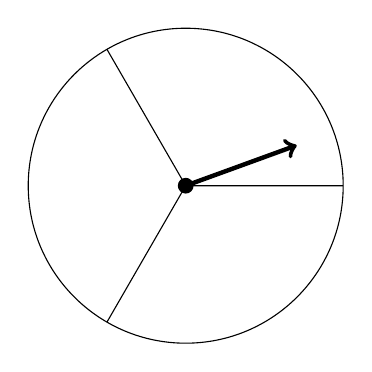
\begin{tikzpicture}
	\fill [black] (0,0) circle(0.1cm);
	\draw (0,0) circle(2cm);
	\draw (0,0) -- (0:2cm) (0,0) -- (120:2cm)  (0,0) -- (-120:2cm);
	\draw[->, ultra thick] (0,0) -- (20:1.5cm);
	\end{tikzpicture}
	\choice 
	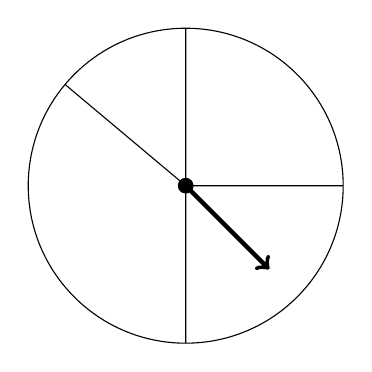
\begin{tikzpicture}
	\fill [black] (0,0) circle(0.1cm);
	\draw (0,0) circle(2cm);
	\draw (0,0) -- (0:2cm) (0,0) -- (90:2cm)  (0,0) -- (140:2cm) (0,0) --  (270:2cm);
	\draw[->, ultra thick] (0,0) -- (-45:1.5cm);
	\end{tikzpicture}
	\choice 
	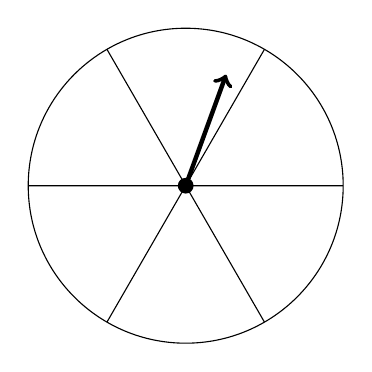
\begin{tikzpicture}
	\fill [black] (0,0) circle(0.1cm);
	\draw (0,0) circle(2cm);
	\draw (0,0) -- (0:2cm) (0,0) -- (60:2cm)  (0,0) -- (120:2cm)  (0,0) -- (180:2cm)  (0,0) -- (240:2cm)  (0,0) -- (300:2cm);
	\draw[->, ultra thick] (0,0) -- (70:1.5cm) ;
	\end{tikzpicture}
	\choice 
	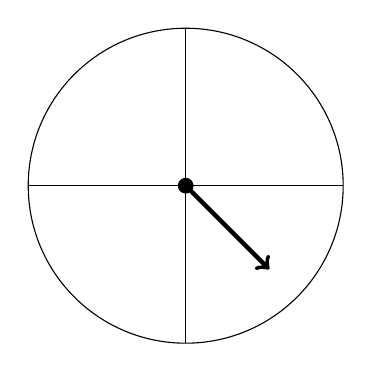
\begin{tikzpicture}
	\fill [black] (0,0) circle(0.1cm);
	\draw (0,0) circle(2cm);
	\draw (0,0) -- (0:2cm) (0,0) -- (90:2cm)  (0,0) -- (180:2cm) (0,0) --  (270:2cm);
	\draw[->, ultra thick] (0,0) -- (-45:1.5cm);
	\end{tikzpicture}	
\end{choices}

\question Wgich fraction is equivalent to 3?
\begin{choices}
	\choice $\frac{1}{3}$
	\choice $\frac{9}{3}$
	\choice $\frac{3}{3}$
	\choice $\frac{8}{4}$
\end{choices}

\newpage
\question Beth met her friend Sally at the library at 3:21pm.  It took Beth 32 minutes to walk from her hom to the library.  What time did beth leave her house to arrive at the library at exactly 4:30pm?

Show your work.
\vskip 8in
\begin{tikzpicture}
\draw (5,0) -- (10,0);
\draw (5,0) node[align=center, left]{Answer:}
\end{tikzpicture}


\end{questions}
\end{document}